\hypertarget{ux6848ux4f8b2ux5386ux53f2ux8fdbux7a0bux6d41ux7a0bux56fe}{%
\section{AI流程图}
\subsubsection{案例:历史进程流程图}\label{ux6848ux4f8b2ux5386ux53f2ux8fdbux7a0bux6d41ux7a0bux56fe}}

\textbf{背景}:梳理``丝绸之路文化交流''中的技术传播路径

\textbf{操作流程}:

\begin{enumerate}
\def\labelenumi{\arabic{enumi}.}
\item
  \textbf{描述需求}
  Prompt:
  \prompt{``用Mermaid语法绘制佛教从印度经中亚传入中国的流程图,包含主要节点和传播方式''}
\item
  \textbf{获得代码} GPT输出:
  
\begin{gptbox}
\small{
\begin{lstlisting}
graph LR
 A[印度那烂陀寺] -->|法显陆路取经| B[龟兹]
 B --> C[敦煌莫高窟]
 A -->|海上丝绸之路| D[广州光孝寺]
 C --> E[长安大雁塔]
 D --> E
\end{lstlisting}
}
\end{gptbox}

\item
  \textbf{实时渲染}:将代码粘贴至Markdown编辑器或Mermaid Live
  Editor,立即生成矢量图
  \fig[h]{
    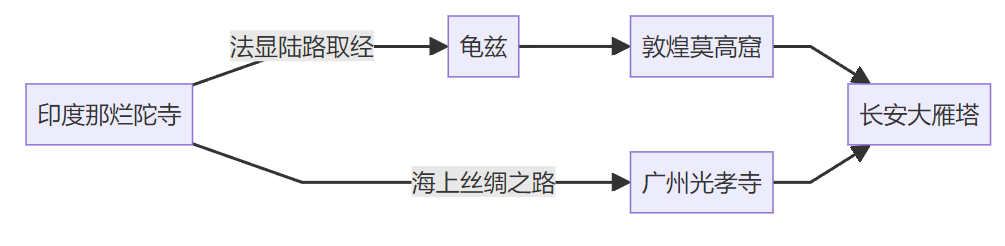
\includegraphics[width=0.7\textwidth]{assets/figures/1739189207681.jpg} %插入图片,[]中设置图片大小,{}中是图片文件名
    \caption{矢量图} %最终文档中希望显示的图片标题
    \label{fig:morse} %用于文内引用的标签
}
\end{enumerate}